\section{Term-Templates}
\label{section:term-templates}

The compile-time representation of terms differs greatly from the runtime representation described previously. The reason for this is the necessity to handle ellipses; or, more specifically, the substitution of pattern variables under ellipses - \texttt{PltRedex} handles this dynamically and erroneous ellipses aren't detected until term creation time.
It is desirable to handle ellipsis depth checking of pattern variables at compile time to be able to provide compile time error messages. Doing this allows for the complete elimination of ellipses from the runtime (with variable \texttt{...} being a reserved symbol that throws an Exception). In addition, this also allows for the detection of metafunction applications statically.

The grammar for terms can be seen in Figure \ref{termtemplate-grammar}. To differentiate between runtime terms, the compile-time representation of terms will be called \textbf{term-templates}.

\begin{figure}
\begin{minted}[tabsize=2,obeytabs,escapeinside=//,mathescape=true,fontsize=\normalsize]{text}
term-template = pattern-variable
              | (term-sequence *)
              |,(functionname term*)
              |(in-hole term term)
              | hole
              | integer
              | float
              | string
              | boolean
term-sequence = term
              | term ... ; literal ellipsis
              | ,@(function term *)
              | ,@(function term *) ...; literal ellipsis
\end{minted}
\caption{Grammar for term-templates.}
\label{termtemplate-grammar}
\end{figure}

\begin{itemize}
\item
\texttt{pattern-variable} represents pattern variables.
\item
\texttt{,(functionname term*)} calls a user-implemented RPython function with zero or more terms as arguments.
\item
\texttt{,@(functionname term*)} calls a user-implemented RPython function with zero or more terms as arguments that must return a list. Contents of the returned list are then inserted into term-sequence at that position.
\item
\texttt{(in-hole term term)} locates \lstinline{hole} in the first term and replaces it with the second term.
\item
\texttt{hole} represents the term \lstinline{hole}
\item
\texttt{integer} represents any literal integer.
\item
\texttt{float} represents any literal floating point number.
\item
\texttt{string}  represents any literal string.
\item
\texttt{boolean}  represents any literal boolean.
\item
\texttt{term-sequence} represents a list of term.  Each individual term within the sequence can be suffixed with ...(literal ellipsis) indicating ellipsis depth of the term-template.
\end{itemize}

\section{Compile-time Representation of Term-Templates}

Throughout the report the following notation will be used to represent actual Python classes used to implement the term-templates.

\begin{figure}[H]
	\centering
	\makebox[\textwidth][c] { 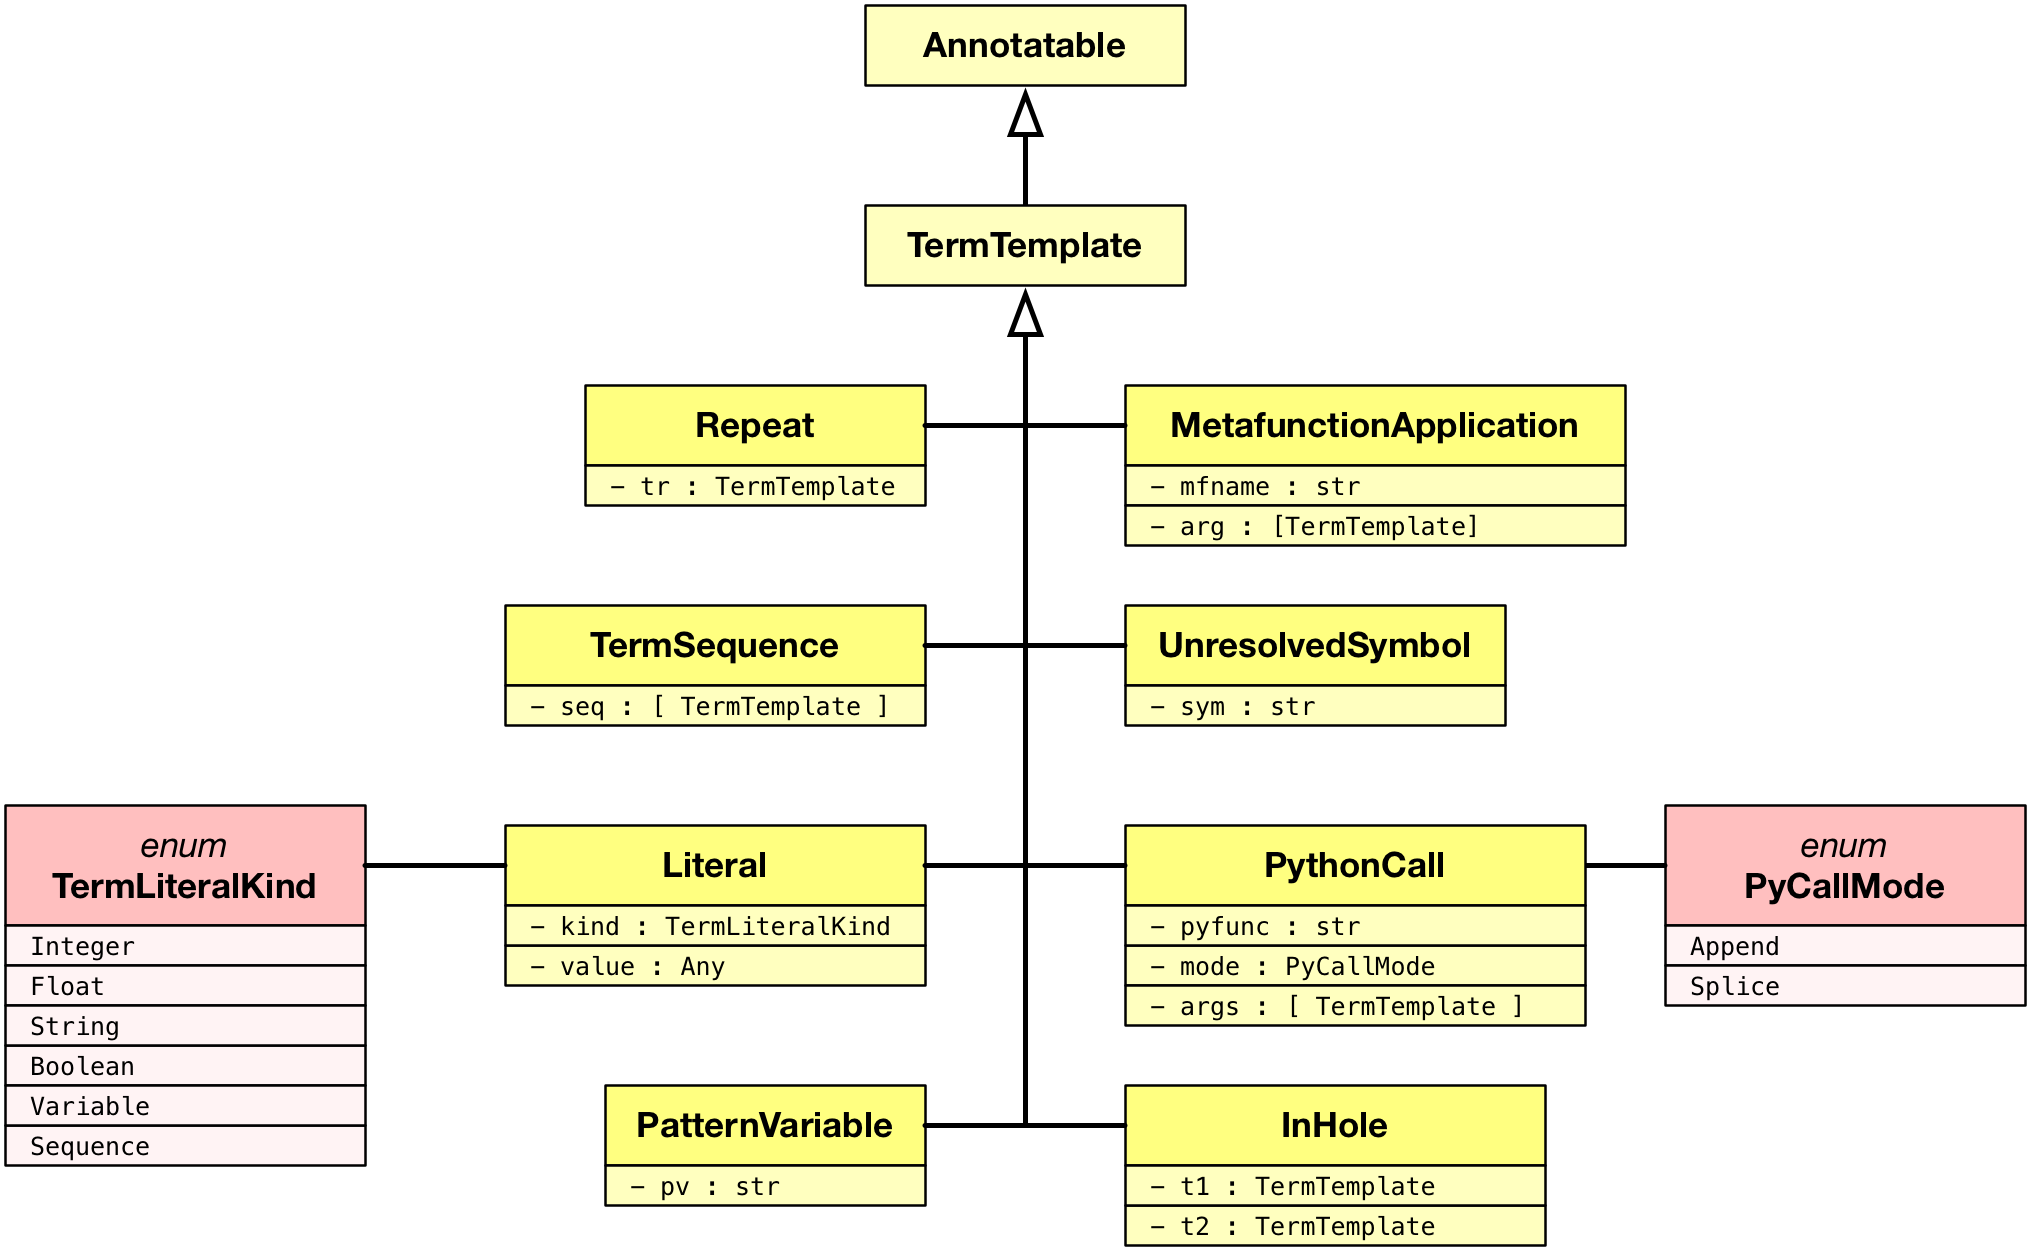
\includegraphics[scale=0.19]{class-diagram-termtemplate.png} }
	\caption{Representation of term-templates.}
\label{class-diagram-termtemplate}
\end{figure}

Figure \ref{class-diagram-termtemplate} shows class diagram for all term-templates.


\begin{itemize}
\item \TermSequence \space represents term sequences and may contain zero or more child term-templates $t_i$.
\item \TermRepeat \space represents term sequence under ellipsis.
\item \TermInHole \space represents \texttt{in-hole} term template
\item \PythonCall \\ represents \texttt{,(functionname term*)} and \texttt{,@(functionname term*)} term-template. $mode$ is used to indicate which one of those it is - $m$ is set to \texttt{Normal} if it is the first, otherwise \texttt{Splice} if it is the latter. $pyfunc$ is expected to be a defined RPython-compatible function.
\item \TermLiteral - represents any literal in term-template. It is initialized with the appropriate tag.
\item \PatternVariable \space represents all pattern variables.
\item \UnresolvedSymbol \space represents unresolved symbols. Initially it is unknown if a symbol is a pattern-variable or a literal.
\end{itemize}
